برای حذف خط میانی حرف $\theta$ و دستیابی به عدد صفر، از عملگر \lr{Opening} با عنصر ساختاری سوم استفاده می‌کنیم:

\begin{flalign*}
SE_3 &= {(0,0), (0,-1)} &&\
A_{\text{eroded}} &= A \ominus SE_3 &&\
A_{\text{opened}} &= A_{\text{eroded}} \oplus SE_3 &&
\end{flalign*}

خط افقی میانی ضخامت عمودی یک پیکسل دارد، در حالی که حلقه‌ها و ستون‌های کناری دارای ضخامت عمودی حداقل دو پیکسل هستند. بنابراین، عملگر سایش با عنصر عمودی ۲ پیکسلی ($SE_3$) تنها خط میانی را کاملاً حذف می‌کند و عملگر بسط در ادامه، سایر بخش‌های تصویر را بدون تغییر به حالت اولیه بازمی‌گرداند.

\begin{center}
\begin{tabular}{cc}
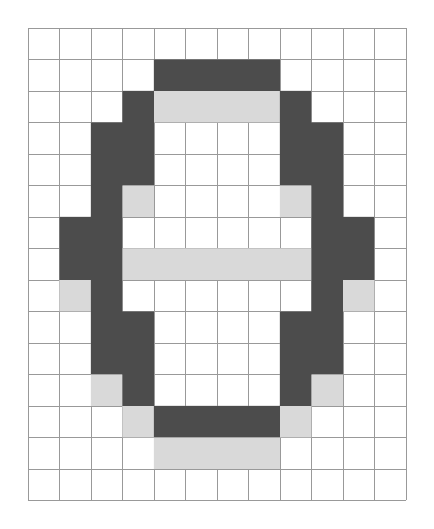
\begin{tikzpicture}[scale=0.4]
\draw[step=1cm,black!40,very thin] (0,0) grid (12,15);
\fill[black!15]
(4,13) rectangle (8,14)
(3,12) rectangle (9,13)
(2,9) rectangle (4,12) (8,9) rectangle (10,12)
(1,6) rectangle (3,9) (9,6) rectangle (11,9)
(3,7) rectangle (9,8)
(2,3) rectangle (4,6) (8,3) rectangle (10,6)
(3,2) rectangle (9,3)
(4,1) rectangle (8,2);
\fill[black!70]
(4,13) rectangle (8,14)
(3,12) rectangle (4,13) (8,12) rectangle (9,13)
(2,11) rectangle (4,12) (8,11) rectangle (10,12)
(2,10) rectangle (4,11) (8,10) rectangle (10,11)
(2,9) rectangle (3,10) (9,9) rectangle (10,10)
(1,8) rectangle (3,9) (9,8) rectangle (11,9)
(1,7) rectangle (3,8) (9,7) rectangle (11,8)
(2,6) rectangle (3,7) (9,6) rectangle (10,7)
(2,5) rectangle (4,6) (8,5) rectangle (10,6)
(2,4) rectangle (4,5) (8,4) rectangle (10,5)
(3,3) rectangle (4,4) (8,3) rectangle (9,4)
(4,2) rectangle (8,3);
\end{tikzpicture}
&
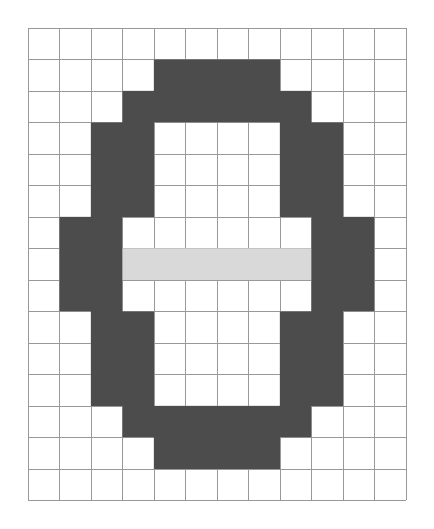
\begin{tikzpicture}[scale=0.4]
\draw[step=1cm,black!40,very thin] (0,0) grid (12,15);
\fill[black!15]
(4,13) rectangle (8,14)
(3,12) rectangle (9,13)
(2,9) rectangle (4,12) (8,9) rectangle (10,12)
(1,6) rectangle (3,9) (9,6) rectangle (11,9)
(3,7) rectangle (9,8)
(2,3) rectangle (4,6) (8,3) rectangle (10,6)
(3,2) rectangle (9,3)
(4,1) rectangle (8,2);
\fill[black!70]
(4,13) rectangle (8,14)
(3,12) rectangle (9,13)
(2,9) rectangle (4,12) (8,9) rectangle (10,12)
(1,6) rectangle (3,9) (9,6) rectangle (11,9)
(2,3) rectangle (4,6) (8,3) rectangle (10,6)
(3,2) rectangle (9,3)
(4,1) rectangle (8,2);
\end{tikzpicture}
\\
$A_{\text{eroded}}$ & $A_{\text{opened}}$
\end{tabular}
\end{center}